\chapter{\difficult{Higher-dimensional Geometry}}\label{chapter:hdg}

    The main references are \cite{higher_gauge, phd_schreiber}. The section on spectral geometry is based on the thesis \cite{spectral_geometry}, while that on smooth spaces is inspired by \cite{baez_convenient}. For an introduction to (higher) category theory, see Chapter \ref{chapter:cat}. Section \ref{section:higher_lie_structures} gives a different approach to the higher-dimensional analogues of Lie algebras.

    In this chapter certain constructions and theorems introduced in the previous chapters are generalized to the setting of higher categories. As such it can been as an analogue to Chapter \ref{chapter:hda} for (differential) geometry.

    ?? CITE BAEZ, SCHREIBER, BARTELS, ... ??

\section{Infinite-dimensional geometry}\label{section:infinie_dimensional}

    In many situations, when consider function spaces, the objects under consideration do not form a finite-dimensional manifold. However, with some care, one can drop this size condition. In Chapter \ref{chapter:functional} it was shown how one can extend calculus from $\mathbb{R}^n$ to infinite-dimensional vector spaces.

    The first approach uses a locally convex TVS \ref{functional:locally_convex} as local model space:
    \newdef{$E$-manifold}{\index{manifold}
        Let $E$ be a locally convex TVS. A Hausdorff topological space is called an $E$-manifold if exists an atlas of charts $(U,\varphi)$, where $\varphi:U\rightarrow\varphi(U)\subset E$ is a homeomorphism and the transition maps are smooth in the sense of Gateaux.
    }

    \newdef{Kinematic tangent bundle}{\index{tangent!bundle}
        Let $M$ be an $E$-manifold with a smooth atlas $\{U_i,\varphi\}_{i\in I}$. The kinematic tangent bundle of $M$ is defined as the quotient of
        \begin{gather}
            \bigsqcup_{i\in I}U_i\times E
        \end{gather}
        by the equivalence relations $(x,w)\sim(x,d\psi_{ji}(\varphi_i(x);v))$.
    }
    \begin{remark}
        For infinite-dimensional $E$, this tangent bundle is not isomorphic to the definition in terms of derivations. The above construction is ``kinematical'' because the pair $(x,v)$ represent a vector tangent to a curve at the point $x\in M$.
    \end{remark}

    Since infinite-dimensional vector are in general not reflexive, simply defining the cotangent bundle to be the fibrewise dual of the kinematic tangent bundle, would lead to even more size issues. \textit{Kriegl} and \textit{Michor} have shown that one can ccok up to 12 sensible definitions of a cotangent bundle (this also includes ``operational'' definitions using derivations). However, only one of these definitions is well-behaved with respect to Lie derivatives, exterior derivatives and pullbacks. Luckily this is also the definition is the most widely used one in the finite-dimensional setting:
    \newdef{Kinematical cotangent bundle}{
        Let $M$ be an $E$-manifold. Consider the set of bounded, alternating linear maps $E^{\times k}\rightarrow\mathbb{R}$. This lifts to a vector bundle $L^k_\mathrm{alt}(TM,M\times\mathbb{R})$, the kinematical cotangent bundle.
    }

\section{Smooth spaces}\index{smooth!space}\label{section:smooth_spaces}

    In this section some generalizations of spaces that are better behaved when considering their properties as a whole are introduced. Before moving to the smooth setting, a bit of history will be given, starting from the ordinary topological setting.

    The first problem in the study of the global properties of spaces arose in algebraic topology. When consider mapping spaces it is sometimes useful to use the currying operation \[C(X\times Y,Z)\rightarrow C(X,C(Y,Z)).\] However, in general, this is not a homeomorphism, i.e.~currying does not define an adjunction and, therefore, $\mathbf{Top}$ is not Cartesian closed \ref{cat:closed}. This problem was treated by \textit{Steenrod} and others, and the solution was simply to restrict to a smaller class of better behaved spaces: the compactly generated Hausdorff spaces.\footnote{This is in general not a problem since all interesting spaces, such as CW complexes, belong to this class.}

    Whilst studying varieties in algebraic geometry people experienced similar problems. For this reason \textit{Grothendieck} invented schemes (see Chapter \ref{chapter:alggeom} and Section \ref{section:schemes} in particular). The main takeaway of this approach was that it is often better to work with a well-behaved category containing some ``nasty'' objects, than to work with a ``nasty'' category containing only nice objects.

    The category $\mathbf{Diff}$ of finite-dimensional smooth manifolds suffers the same problems, namely the space of smooth functions $C^\infty(X,Y)$ is in general some kind of infinite-dimensional manifold. It becomes even worse if one studies the mapping spaces between those. \textit{Kriegl} and \textit{Michor} have introduced a framework in which one can work safely, but the main problem with their solution is that not all spaces of interest are included. Certain other operations such as quotients and (co)limits are also not guaranteed to exist within that category.

\subsection{Concrete sites}

    \newdef{Diffeological space}{\index{diffeology}\index{plot}
        Let $X$ be a set. A diffeology $\mathcal{D}$ on $X$ is defined as a collection of functions $f:U\subseteq\mathbb{R}^n\rightarrow X$, called \textbf{plots}, satisfying the following conditions (where $U,V$ and $W$ are open sets):
        \begin{enumerate}
            \item If $f$ is constant, then $f\in\mathcal{D}$. Equivalently, every function $f:\mathbb{R}^0\rightarrow X$ is a plot.
            \item If $\{U_i\}_{i\in I}$ is an open cover of $U$ and if $f|_{U_i}\in\mathcal{D}$ for all $i\in I$, then $f\in\mathcal{D}$.
            \item If $f\in\mathcal{D}$ and $g:W\subseteq\mathbb{R}^m\rightarrow\dom(f)$ is smooth, then $f\circ g\in\mathcal{D}$.
        \end{enumerate}
        The set $X$ can be turned into a topological space by equipping it with the \textbf{$\mathcal{D}$-topology}, i.e.~the final topology with respect to $\mathcal{D}$.
    }
    \remark{The domain of different plots can be subsets of different Euclidean spaces $\mathbb{R}^m$ and $\mathbb{R}^n$.}

    \newdef{Smooth map}{\index{smooth!function}
        \nomenclature[S_DiffSp]{$\mathbf{DiffSp}$}{category of diffeological spaces and smooth maps}
        Let $(X,\mathcal{D})$ and $(Y,\mathcal{D}')$ be diffeological spaces. A map $g:X\rightarrow Y$ is said to be smooth if for every $f\in\mathcal{D}$ the composition $g\circ f\in\mathcal{D}'$.

        The diffeological spaces together with their differentiable morphisms form a category $\mathbf{DiffSp}$.
    }

    \newdef{Chen space}{\index{Chen space}
        If the open sets in the definition of a diffeological space are replaced by convex sets, the notion of smooth spaces due to \textit{Chen} are obtained.
    }

    \begin{adefinition}[Manifold]\index{manifold}
        A diffeological space is called an $n$-manifold if it is locally diffeomorphic to a Euclidean space. A map between manifolds is smooth in the diffeological sense if and only if it smooth in the sense of Definition \ref{manifolds:smooth_function}.
    \end{adefinition}

    There exist two trivial smooth structures:
    \begin{example}[Discrete structure]\index{discrete!smooth structure}
        The smooth structure defined by taking the plots to be the constant functions.
    \end{example}
    \begin{example}[Indiscrete structure]
        The smooth structure obtained by taking all functions to be plots.
    \end{example}

    \newdef{Smooth set}{\index{smooth!set}
        \nomenclature[S_Cinf]{$\mathbf{C^\infty}$}{category of smooth spaces}
        By omitting the reference to an underlying set in the definition of smooth spaces above, a more general definition can be obtained. This way the category $\mathbf{SmoothSet}$ is obtained as the sheaf category on the site of Cartesian spaces $\mathbf{Sh(CartSp_{diff})}$. The topology on this site is generated by the coverage of differentiably good covers \ref{manifold:good_cover} (in fact, this topology coincides with the usual one consisting of open covers). Diffeological spaces can be recovered by passing to the full subcategory on \textit{concrete sheafs}. The category of smooth spaces/sets is often denoted by $\mathbf{C^\infty}$.

        ?? ADD INFORMATION ON CONCRETE SHEAFS ??
    }

    \begin{example}[Differential forms]
        Consider the $k^{th}$ de Rham functor $\Omega^k$ on the category $\mathbf{Diff}$. This functor assigns to every smooth manifold its space of differential $k$-forms (Section \ref{section:forms}). Locally defined forms can be glued together if they agree on intersections and, hence, they satisfy the sheaf condition. This shows that $\Omega^k$ is a smooth space, albeit one that is far from an ordinary smooth manifold.

        One can go even further. Consider the subfunctor $\Omega^2_\mathrm{cl}$ that assigns closed two-forms to a smooth manifold. This also defines a smooth space and, hence, one can consider the slice category $\mathbf{C^\infty}/\Omega^2_\mathrm{cl}$. It is not hard to show that the category $\mathbf{SpMfd}$ of symplectic manifolds admits an embedding into this slice category.
    \end{example}

    \begin{property}
        There exists an adjunction
        \begin{gather}
            \mathbf{Top}\adj{top}{\text{\textit{diff}}}\mathbf{C^\infty}.
        \end{gather}
        The functor $\text{\textit{diff}}$ endows a topological space $X$ with the smooth structure for which every continuous map $U\rightarrow X$ is a plot. The adjoint functor $top$ sends a smooth space to the topological space equipped with the finest topology for which all plots become continuous maps.
    \end{property}

    \newdef{Smooth algebra}{\index{smooth!algebra}
        \nomenclature[S_CSmAlg]{$\mathbf{C^\infty Ring},\mathbf{C^\infty Alg}$}{category of smooth algebras}
        For any smooth manifold $M$ the algebra of smooth functions can be obtained as a hom-object: \[C^\infty(M)\equiv C^\infty(M,\mathbb{R}) = \mathbf{Diff}(M,\mathbb{R}).\] Since hom-functors are (finite) product-preserving, one can see that the multiplication $C^\infty(M)\times C^\infty(M)\rightarrow C^\infty(M)$ is induced by the multiplication on $\mathbb{R}$: \[C^\infty(M, \mathbb{R}\times\mathbb{R})\cong C^\infty(M)\times C^\infty(M).\] Furthermore, the hom-functor is covariant in the second argument and, hence, a copresheaf on the category $\mathbf{CartSp_{diff}}$ of Euclidean (Cartesian) spaces and smooth morphisms is obtained. Generalizing this situation, smooth algebras are defined as finite product-preserving copresheaves on $\mathbf{CartSp_{diff}}$. This (functor) category is denoted by $\mathbf{C^\infty Alg}$.

        Given a smooth algebra $R$, its \textbf{underlying algebra} $U(R)$ is defined as the set $R(\mathbb{R})$ equipped with the canonically induced ring operations.
    }
    \newdef{Finitely generated smooth algebra}{
        Since ordinary $R$-algebras are finitely generated if and only if they are of the form $R[x_1,\ldots,x_k]/J$ for some integer $k\in\mathbb{N}$ and some ideal $J$, a smooth algebra is said to be finitely generated if it is of the form $C^\infty(\mathbb{R}^n)/J$ for some $n\in\mathbb{N}$ and some ideal $J$ in the ordinary ring underlying the smooth algebra.
    }
    \newdef{Smooth locus}{\index{smooth!locus}
        Let $\mathbf{C^\infty Alg^{fin}}$ denote the category of finitely generated smooth algebras. The category of \textbf{smooth loci} is defined as $(\mathbf{C^\infty Alg^{fin}})^{op}$. The smooth locus corresponding to a smooth algebra $R$ is often denoted by $\ell R$.
    }

\subsection{Supergeometry}

    In this section the definition of smooth spaces (and sets) is generalized to the odd (fermionic) sector, i.e.~``super smooth sets'' will be defined.
    \newdef{Infinitesimally thickened space}{\index{thickened space}
        \nomenclature[S_FormalCartSp]{$\mathbf{FormalCartSp_{diff}}$}{category of infinitesimally thickened Euclidean spaces}
        First, consider a point $\mathbb{R}^0$. Its infinitesimal thickening should be a space such that every function that vanishes at the origin is actually nilpotent (this is essentially a version of the Kock-Lawvere axiom \ref{synth:kock_lawvere_axiom}). The straightforward definition is the following one:
        \begin{gather}
            \mathbb{D} := \mathrm{Spec}(A),
        \end{gather}
        where $A:=\mathbb{R}\oplus V$ with $V$ a finite-dimensional nilpotent ideal. A Euclidean space can be infinitesimally thickened by taking the product with $\mathbb{D}$ (or at the algebraic level by taking the tensor product with $A$). A morphism of such spaces is defined by an $R$-algebra homomorphism between their assciated algebras. These form the category $\mathbf{FormalCartSp_{diff}}$.
    }
    \begin{example}[First-order neighbourhood]
        By taking $A=\mathbb{R}[\varepsilon]/\varepsilon^2$ one exactly obtains the first-order infinitesimal neighbourhood of Definition \ref{synth:infinitesimal_line}. The morphism dual to the mapping implied by the Kock-Lawvere axiom \ref{synth:kock_lawvere_axiom} gives an inclusion map $\mathbb{D}^1\hookrightarrow\mathbb{R}^1$. (This example can easily be generalized to $k^{th}$-order neighbourhoods.)
    \end{example}

    \begin{property}[Morphisms]
        First, consider the morphisms from a Euclidean space into an infinitesimal neighbourhood $\mathbb{D}^k$. Since such morphisms are dual to algebra homomorphisms, one should look at homomorphisms of the form $\mathbb{R}[\varepsilon]/\varepsilon^{k+1}\rightarrow C^\infty(\mathbb{R}^n)$. However, being an algebra homomorphism implies that $f(1)=1$ and that nilpotents are mapped to nilpotents. The algebra of smooth functions on a Euclidean space does not contain nilpotents and, hence, there exists a unique function into an infinitesimal neighbourhood (the one that factorizes through the one-point set).

        For morphisms out of (first-order) infinitesimal neighbourhoods one obtains the property known from synthetic geometry that morphisms of the form $\mathbb{R}^n\times\mathbb{D}^1\rightarrow\mathbb{R}^n$ are in bijection with vector fields on $\mathbb{R}^n$.
    \end{property}

    \newdef{Formal smooth set}{\index{formal set}\index{smooth|seealso{formal}}\index{Cahiers topos}\index{plot}
        A sheaf on the site of infinitesimally thickened Euclidean spaces (covers are of the form $\{U_i\times\mathrm{Spec}(A)\mid U_i\hookrightarrow\mathbb{R}^n\}$). The category of formal smooth sets or, equivalently, the sheaf topos on $\mathbf{FormalCartSp_{diff}}$ is also called the \textbf{Cahiers topos}. The sets in the image of a formal smooth set $X$ are called the sets of \textbf{plots} of $X$ and can be interpreted as sets of functions into $X$ (in analogy with the definition of smooth spaces).
    }
    \newdef{Reduction}{\index{reduction}\index{infinitesimal}
        Given an infinitesimally thickened space $\mathbb{R}^n\times\mathbb{D}$, its reduction $\mathfrak{R}$ is defined to be $\mathbb{R}^n$. Every reduction induces a canonical morphism $\mathbb{R}^n\hookrightarrow\mathbb{R}^n\times\mathbb{D}$. Plots get can be reduced by ``precomposing'' with a reduction morphism.

        The \textbf{infinitesimal neighbourhood} (to arbitrary order) of a formal smooth subset $Y\hookrightarrow X$ is defined by taking its plots to be those plots of $X$ for which the reductions factorize through plots of $Y$.
    }
    \newdef{Shape modality}{\index{shape}\index{de Rham!shape}
        The infinitesimal shape or \textbf{de Rham shape} $\mathfrak{J}X$ of a formal smooth set $X$ is defined as the formal smooth set obtained by reducing the plots of $X$:
        \begin{gather}
            \mathfrak{J}X(U) := X(\mathfrak{R}(U)).
        \end{gather}
        For its incarnation as a modal operator, see Section \ref{section:modal_type_theory}.
    }

    In analogy to Definition \ref{topology:etale_morphism} one can also define local diffeomorphisms between formal smooth sets:
    \newdef{Local diffeomorphism\footnotemark}{\index{local!diffeomorphism}
        \footnotetext{Also called a \textbf{(formally) \'etale morphism}.}
        A morphism of formal smooth sets $f:X\rightarrow Y$ such that the thickened plots of $X$ can be identified with those of $Y$ whose reduction comes from a Euclidean plot of $X$. More elegantly (or abstractly) this means that the naturality square of the shape modality (interpreted as a monad) forms a pullback square:
        \begin{gather*}
            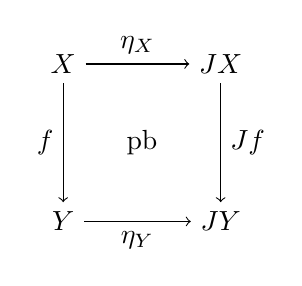
\begin{tikzpicture}
                \node (PB) at (0, 0) {pb};
                \node (X) at (-1, 1) {$X$};
                \node (JX) at (1, 1) {$\mathfrak{J}X$};
                \node (Y) at (-1, -1) {$Y$};
                \node (JY) at (1, -1) {$\mathfrak{J}Y$};
                \draw[->] (X) -- node[above]{$\eta_X$} (JX);
                \draw[->] (Y) -- node[below]{$\eta_Y$} (JY);
                \draw[->] (X) -- node[left]{$f$} (Y);
                \draw[->] (JX) -- node[right]{$\mathfrak{J}f$} (JY);
            \end{tikzpicture}
        \end{gather*}
    }

    \newadef{Smooth manifold}{\index{manifold}
        A diffeological space (in its incarnation as a smooth formal set) equipped with a family of local diffeomorphisms from Euclidean spaces (also regarded as formal smooth sets) such that every point of the space lies in the image of at least one such morphism and such that the final topology induced by the plots of the smooth set is paracompact Hausdorff.
    }

    Although this section started with the promise that spaces would be generalized to the fermionic setting, only bosonic spaces were constructed up to this point. However, everything introduced in this section was formulated in such a way that supergeometry can be included through a minor modification:
    \newdef{Superpoint}{\index{super-!point}\index{super-!space}
        A space of the form $\mathrm{Spec}(A)$ for $A:=\mathbb{R}\oplus V$ with $V$ a finite-dimensional superalgebra \ref{hda:superalgebra} that forms a nilpotent ideal of $A$. When $A$ is taken to be the Grassmann algebra \ref{vector:exterior_algebra} on $n$ generators, the odd point $\mathbb{R}^{0|n}$ is obtained. The \textbf{super Euclidean space} $\mathbb{R}^{m|n}$ is obtained as the product of an ordinary Euclidean space $\mathbb{R}^m$ and the superpoint $\mathbb{R}^{0|n}$, i.e.~its algebra of smooth functions is $C^\infty(\mathbb{R}^m\times\Pi\mathbb{R}^m)$.
    }
    \newdef{Super smooth set}{\index{smooth!set}
        A sheaf on the category of super Euclidean spaces $\mathbf{SuperCartSp_{diff}}$.
    }

\subsection{Graded manifolds}

    In this section some of the notions from Part \ref{part:diffgeom} will be generalized to supermanifolds and general graded manifolds. The general notation $(x^i)$ will be used for the collection of both even and odd coordinates.

    \begin{example}[Supermanifold]\index{super-!manifold}
        A super smooth set in the form of a locally ringed space $(M,\mathcal{A})$ that is locally isomorphic to a super Euclidean space, i.e.~$\mathcal{A}$ is locally given by $C^\infty(M)\otimes\Lambda^\bullet\mathbb{R}^n$ for some $n\in\mathbb{N}$. More generally, a \textbf{graded manifold} is a locally ringed space that is locally isomorphic to $(\mathbb{R}^m, C^\infty(\mathbb{R}^m)\otimes\Sym(V^*))$ for a graded vector space $V$. (A supermanifold can be recovered by taking $V=\Pi\mathbb{R}^n$.)
    \end{example}

    \begin{theorem}[Batchelor]
        Let $(M,\mathcal{A})$ be an $\mathbb{N}$-graded manifold. There exists a vector bundle $E\rightarrow M$ such that $\mathcal{A}$ is isomorphic to the structure sheaf $\Gamma(\Lambda^\bullet E)$, i.e.~$\mathcal{A}$ is locally given by $\Sym(\Lambda^\bullet E^*)$. If $(M,\mathcal{A})$ is a supermanifold, there exists a vector bundle $E\rightarrow N$ such that $\mathcal{A}$ is locally given by $\Lambda^\bullet E^*$.
    \end{theorem}

    \newdef{Vector field}{\index{vector field}
        A graded vector field of degree $k$ is a degree-$k$ derivation on $C^\infty(M)$. The integer $k$ is called the \textbf{degree}.
    }
    \newdef{Cohomological vector field}{\index{vector field!cohomological}
        A graded vector field $X$ of degree $1$ that satisfies $[X,X]=0$. Every degree-1 graded vector field satisfies
        \begin{gather}
            [X,X] = 2X\circ X,
        \end{gather}
        which implies that every cohomological vector field defines a coboundary operator on $C^\infty(M)$. A graded manifold equipped with a cohomological vector field is called a \textbf{differential-graded manifold} (dg-manifold).
    }
    \begin{example}[de Rham differential]
        Consider the de Rham complex $\Omega^\bullet(M)$ with differential $d$. This differential corresponds to a cohomological vector field $Q$ on $\Pi TM$, locally defined by
        \begin{gather}
            Q := \sum_{i=1}^n\drx^i\partial_i.
        \end{gather}
        Note that the differentials $dx^i$ are here regarded as coordinate functions on $\Pi TM$. The \textbf{degree} of a homogeneous element of $\Omega^\bullet(M)$ is defined as the difference of its graded degree and its form degree. The de Rham complex itself then corresponds to the algebra $C^\infty(\Pi TM)$.
    \end{example}

    \newdef{Poisson manifold}{\index{Poisson!manifold}\label{hdg:poisson_manifold}
        Consider a degree-$k$ symplectic form $\omega$. This form induces a Poisson structure on the algebra $C^\infty(M)$ as follows:
        \begin{gather}
            \{f,g\} := (\partial^R_if)\omega^{ij}(\partial^L_jg).
        \end{gather}
        It is not hard to check that this operation is graded-commutative. As in Section \ref{section:hamiltonian_vector_fields}, a Hamiltonian vector field can be defined for any smooth function $H\in C^\infty(M)$:
        \begin{gather}
            \omega(X_H,\cdot) = -\dr H(\cdot).
        \end{gather}
    }

    \begin{property}[Euler vector field]\index{Cartan!magic formula}\index{Lie!derivative}\index{Euler!homogeneous function theorem}
        Consider the graded vector field
        \begin{gather}
            E := \sum_{i=1}^n\deg(x^i)x^i\partial_i.
        \end{gather}
        The Lie derivative $\mathcal{L}_E$, defined through the Cartan formula
        \begin{gather}
            \mathcal{L}_E := \iota_E\dr + (-1)^{\deg(E)}\dr\iota_E,
        \end{gather}
        acts on homogeneous forms by multiplication by their degree.
    \end{property}
    \begin{property}\index{Hamiltonian!vector field}\label{hdg:global_exactness}
        Every closed differential form of degree $k\neq0$ is exact. More generally, the de Rham cohomology of a graded manifold is isomorphic to the de Rham cohomology of its body. This for example implies that a degree-$l$ symplectic vector field $X$ is Hamiltonian with respect to a degree-$k$ symplectic form if $k+l\neq0$.
    \end{property}
    \begin{result}[dg-symplectic manifold]\index{master equation}
        Consider a Hamiltonian cohomological vector field $X$. There exists a Hamiltonian function $H$ such that
        \begin{gather}
            Xf = \{H,f\}
        \end{gather}
        for all $f\in C^\infty(M)$. If the symplectic form has degree $k$, the function $H$ can be chosen to be of degree $k+1$ and, accordingly, $\{H,H\}$ will be of degree $k+2$. Now, the identity $[X,X] = 0$ also implies that $\{H,H\}$ is a constant and, since all constants are of degree 0, it follows that
        \begin{gather}
            \label{hdg:classical_master_equation}
            \{H,H\}=0
        \end{gather}
        whenever $k\neq-2$. This equation is often called the \textbf{classical master equation}. A graded manifold equipped with both a symplectic form and a symplectic cohomological vector field is called a \textbf{differential-graded symplectic manifold}.

        If $\omega$ is of degree 1, it was shown by \textit{Schwarz} that $(M,\omega)$ is symplectomorphic to $\Pi T^*M$ such that the Poisson bracket is mapped to the Schouten-Nijenhuis bracket and the Hamiltonian is mapped to a Poisson bivector field exactly if it satisfies the master equation.
    \end{result}

\subsection{Gauge theory}

    Recall the notions of Chapter \ref{chapter:topos}, in particular the notions of stacks and higher topoi. The $(\infty,1)$-category of smooth $\infty$-stacks can be described in terms of (left Bousfield) localization of a suitable presheaf category by Lurie's theorem \ref{model:lurie_presentation}.

    The first possibility is the category of $\infty$-presheaves on $\mathbf{Diff}$ with the localization at open covers. While, the second possibility is the dense subsite $\mathbf{CartSp}_\mathrm{diff}$ with localization at good open covers. Both will result in a \v{C}ech model structure \ref{topos:cech_model_structure}. However, the exact properties will differ.

    \begin{example}[Classifying stacks]
        Consider the example of a Lie group $G$ and its classifying stack $\mathbf{B}G$. In the first model structure, the mapping space $\mathbf{H}(M,\mathbf{B}G)$, for $M$ a smooth manifold, is just presented\footnote{This means the homotopy-invariant hom-object in the underlying presheaf category, where the domain is replaced by a cofibrant object and the codomain by a fibrant object.} by $\hom(M,\mathbf{B}G)$, since $M$ is cofibrant as a representable presheaf and $\mathbf{B}G$ is fibrant by gluing over covers. So mapping spaces $\mathbf{H}(M,\mathbf{B}G)$ are just given by groupoids of $G$-bundles over $M$.

        On the subsite $\mathbf{CartSp}_\mathrm{diff}$, the presheafs represented by manifolds are not cofibrant anymore. However, \v{C}ech nerves of open covers give a cofibrant replacement. On the other hand, over Cartesian spaces the stacks are trivial and can be presented as action groupoids $\ast/\!\!/G$ (the ordinary deloopings). A fibrant replacement is given by the presheaf
        \begin{gather}
            U\mapsto N_\Delta(\ast/\!\!/C^\infty(U,G)).
        \end{gather}
        This presheaf is also equivalent to the groupoid of $G$-bundles (over $U$). The derived mapping space in this situation is given by (normalized) $G$-valued \v{C}ech cocycles.
    \end{example}

\section{Higher geometry}

    In this section some notions about groups, Lie groups and groupoids (Sections \ref{section:groups}, \ref{section:lie_groups} and \ref{section:groupoids}) are extended the setting of higher category theory.

\subsection{Groups}

    \newdef{Lie groupoid\footnotemark}{\index{Lie!groupoid}\label{hdg:lie_groupoid}
        \footnotetext{In a similar way one could define \textit{topological groupoids, \'etal\'e groupoids}, ...}
        A groupoid internal to $\mathbf{Diff}$.

        Note that Definition \ref{cat:internal_category} requires the existence of pullbacks. In the category $\mathbf{Diff}$ this is equivalent to assuming that the source and target morphisms are (surjective) submersions.
    }
    \remark{In the Ehresmannian approach one gives the manifold of composable morphisms $D_1\times_{D_0}D_1$ as part of the data. Hence, no further assumptions have to be made about the source and target morphisms.}

    \newdef{Lie algebroid}{\index{Lie!algebroid}\index{anchor}\label{hdg:lie_algebroid}
        A vector bundle $\pi:E\rightarrow M$ together with a vector bundle morphism $\rho:E\rightarrow TM$, called the \textbf{anchor map}, and a Lie bracket on $\Gamma(E)$ such that the following Leibniz-type property is satisfied:
        \begin{gather}
            [X,fY] = f[X,Y] + \rho(X)(f)Y.
        \end{gather}
        This property also implies that $\rho$ preserves the Lie bracket:
        \begin{gather}
            \rho([X,Y]) = [\rho(X),\rho(Y)].
        \end{gather}
        In local coordinates $x^i$ and for a local basis of sections $s_\alpha$, the bracket and anchor can be expressed in terms of structure functions:
        \begin{align}
            \rho(s_\alpha) &= R^i_\alpha\partial_i\\
            [s_\alpha,s_\beta] &= C^\gamma_{\alpha\beta}(x)s_\gamma.
        \end{align}
        The Lie algebroid properties then imply the following conditions on these structure functions:
        \begin{gather}
            R^j_\alpha\pderiv{R^i_\beta}{x^j}-R^j_\beta\pderiv{R^i_\alpha}{x^j} = R^i_\gamma C^\gamma_{\alpha\beta}
        \end{gather}
        and
        \begin{gather}
            R^i_\alpha\pderiv{C^\kappa_{\beta\gamma}}{x^i}+C^\kappa_{\alpha\mu}C^\mu_{\beta\gamma} + (\alpha\leftrightarrow\beta\leftrightarrow\gamma) = 0.
        \end{gather}
    }
    \begin{example}[Tangent Lie algebroid]\index{pair!groupoid}
        The tangent bundle over a smooth manifold is a Lie algebroid with $\rho\equiv\mathbbm{1}_{TM}$.

        Consider the \textbf{pair groupoid} $\mathbf{M\times M}$, i.e.~the groupoid with the following data:
        \begin{itemize}
            \item\textbf{Objects}: $M$
            \item\textbf{Morphisms}: $M\times M$, i.e.~between every two points there exists a unique morphism.
        \end{itemize}
        Both the fundamental groupoid $\mathbf{\Pi_1}(M)$ (Definition \ref{topology:fundamental_groupoid}) and the pair groupoid $\mathbf{M\times M}$ integrate the tangent Lie algebroid.
    \end{example}

    One can generalize the dual construction of $L_\infty$-algebras \ref{hda:l_infinity_bis} even further:
    \newdef{$L_\infty$-algebroid}{
        Consider the construction of the Chevalley-Eilenberg algebra for a $L_\infty$-algebra. By replacing the base field by a smooth algebra $C^\infty(M)$ for some smooth manifold $M$ and the (graded) vector space $V$ by a module of sections $\Gamma(E)$ of a (graded) vector bundle $E\rightarrow M$, one obtains the notion of a $L_\infty$-algebroid.
    }
    \begin{property}
        $L_\infty$-algebras can be recovered by considering the special case $M=\{\ast\}$.
    \end{property}

    \begin{example}[de Rham complex]\index{de Rham!complex}
        Consider the tangent algebroid of a smooth manifold $M$. The associated Chevalley-Eilenberg complex is equivalent to the de Rham complex $\Omega^\bullet(M)$.
    \end{example}

    \newdef{Weak 2-group}{\index{group!categorical}\index{2-!group}
        Let $(\mathbf{C},\otimes,\mathbf{1})$ be a monoidal category. This category is called a weak 2-group, \textbf{categorical group} or \textbf{gr-category} if it satisfies the following conditions:
        \begin{enumerate}
            \item All morphisms are invertible.
            \item Every object is weakly invertible with respect to the monoidal structure.
        \end{enumerate}
        By Property \ref{cat:monoidal_or_2} one can equivalently define a weak 2-group as a 2-category with a single object, weakly invertible 1-morphisms and invertible 2-morphisms.
    }
    \newdef{2-groupoid}{\index{2-!groupoid}
        A 2-groupoid is a 2-category in which all 1-morphisms are invertible and every 2-morphisms has a ``vertical'' inverse. (The ``horizontal'' inverse can be constructed from the other ones.)
    }
    \newdef{Strict 2-group}{
        A (strict) 2-group is defined as a (strict) 2-groupoid with only one object. From this it follows that the set of 1-morphisms forms a group and so does the set of 2-morphisms under horizontal composition. However, the 2-morphisms do not form a group under vertical composition because the sources/targets may not match.

        This definition is equivalent to the following internal version. A (strict) 2-group is a group object in $\mathbf{Cat}$ or an internal category in $\mathbf{Grp}$. If $\mathbf{Grp}$ is replaced by $\mathbf{Lie}$, the notion of a (strict) Lie 2-group is obtained.
    }
    \newdef{$\infty$-groupoid}{
        A $\infty$-category in which all morphisms are invertible. This is equivalent to a $(\infty,0)$-category in the language of $(n,r)$-categories.
    }

    \begin{property}[Lie crossed modules]\index{module!crossed}\index{differential!crossed module}
        The 2-category of (strict) 2-groups is biequivalent to the 2-category of (Lie) crossed modules \ref{group:crossed_module}. Given a 2-group $\mathcal{G}$, a crossed module is obtained as follows:
        \begin{itemize}
            \item $G:=\ob{\mathcal{G}}$,
            \item $H:=\{h\in\mathrm{hom}(\mathcal{G})\mid\mathfrak{s}(f)=e\}$,
            \item $t(h):=\mathfrak{t}(h)$, and
            \item $\alpha(g)h := \mathbbm{1}_gh\mathbbm{1}_g^{-1}$,
        \end{itemize}
        where $\mathfrak{s},\mathfrak{t}$ are the source and target morphisms in $\mathcal{G}$.

        To every Lie crossed module one can also assign a \textbf{differential crossed module}. This consists of the following data:
        \begin{itemize}
            \item two Lie algebras $\mathfrak{g},\mathfrak{h}$,
            \item a Lie algebra morphism $\partial:\mathfrak{h}\rightarrow\mathfrak{g}$, and
            \item a Lie algebra morphism $\rho:\mathfrak{g}\rightarrow\text{Der}(\mathfrak{h})$.
        \end{itemize}
        The equivariance and Peiffer conditions induce similar conditions for the above data:
        \begin{itemize}
            \item $\partial(\rho(h)g) = [h,\partial g]$, and
            \item $\rho(\partial h)(h') = [h,h']$,
        \end{itemize}
        where $g\in\mathfrak{g}$ and $h,h'\in\mathfrak{h}$. The biequivalence of crossed modules and strict 2-groups induces a biequivalence of differential crossed modules and strict Lie 2-algebras.
    \end{property}

    \begin{example}[Automorphism 2-group]
        Given a Lie group $H$, one can construct a crossed module with $G:=\Aut(H)$, $t$ assigning inner automorphisms (conjugations) and $\alpha$ the obvious map. The associated 2-group $\mathrm{AUT}(H)$ gives a 2-group of symmetries of $H$, i.e.~it is the automorphism 2-group of $H$ in the 2-category $\mathbf{Lie}$.
    \end{example}

    \newdef{Exponentiable group}{\index{exponentiable}
        A smooth group for which every smooth function $f:[0,1]\rightarrow\mathfrak{g}$ corresponds to a smooth function $g:[0,1]\rightarrow G$ such that
        \begin{gather}
            \deriv{}{t}g(t) = f(t)g(t)
        \end{gather}
        with $g(0) = e$. A smooth 2-group is said to be exponentiable if both of its component groups are exponentiable. Since all Lie groups are exponentiable, all Lie 2-groups are also exponentiable
    }

    \begin{remark}[Lie's third theorem]\index{Lie!third theorem}
        In ordinary Lie theory Lie's third theorem states that every (finite-dimensional) Lie algebra can be obtained as the infinitesimal version of a Lie group. However, this does not carry over to the 2-group setting. Consider for example the Lie 2-algebras $\mathfrak{g}_\lambda$ constructed in Example \ref{hda:gk_lie_2_algebra}. As shown in \cite{HDA5} only $\mathfrak{g}_0$ gives rise to a Lie 2-group (or even a topological 2-group).
    \end{remark}

\subsection{Spaces}

    To overcome the problem encountered in Definition \ref{hdg:lie_groupoid} above, one should pass from $\mathbf{Diff}$ to $\mathbf{C^\infty}$. It can be shown that this category admits all pullbacks, quotients, path spaces, etc.

    \newdef{Smooth 2-space}{
        A category internal to $\mathbf{C^\infty}$.

        In the remainder of this chapter all spaces will be assumed to be smooth in this general sense. The notions of 2-groups as introduced in the previous section are easily generalized to this more general setting.
    }

    \newdef{2-group action}{\index{group!action}
        Consider a smooth 2-group $\mathcal{G}$ and a smooth 2-space $E$. A strict action of $\mathcal{G}$ on $E$ is a smooth homomorphism $\mathcal{G}\rightarrow\mathrm{AUT}(E)$, i.e.~a smooth map preserving products and inverses.
    }

    \newdef{Thin homotopy}{\index{homotopy!thin}
        Let $M$ be a smooth manifold. A smooth homotopy $H:[0,1]^2\rightarrow M$ is said to be thin if
        \begin{gather}
            H(s,t) = F(s)
        \end{gather}
        for some smooth $F$ near $t=0,1$ and if it pulls back every two-form to 0:
        \begin{gather}
            \forall\omega\in\Omega^2(M): H^*\omega = 0.
        \end{gather}
    }
    \newdef{Lazy path}{\index{path!lazy}\index{sitting instants}
        Let $M$ be a smooth manifold. A path $f:[0,1]\rightarrow M$ is said to be lazy (or to have \textbf{sitting instants}) if it is locally constant on some neighbourhoods of $0$ and $1$.
    }

    \newdef{Path groupoid}{\index{groupoid!path}\label{hdg:path_groupoid}
        Let $M$ be a smooth space. The path groupoid $\mathcal{P}_1(M)$ is the smooth groupoid conssting of the following data:
        \begin{itemize}
            \item\textbf{Objects}: $M$
            \item\textbf{Morphisms}: thin homotopy classes of lazy paths with fixed endpoints on $M$
        \end{itemize}
        The laziness combined with the first condition of thin homotopies implies that the morphisms of this groupoid are (locally) constant near the full boundary of their domain.

        In fact, by suitably generalizing the smoothness properties of the homotopies and paths, one can extend this definition to surfaces, volumes and so on. This results in the $n$-path $n$-groupoid $\mathcal{P}_n(M)$.
    }
    \remark{The restriction to lazy paths is required to ensure the smoothness of composite paths. The quotient by thin homotopies is required to ensure the validity of the associativity and invertibility properties.}

    ?? COMPLETE ??

\section{2-Bundles}

    A first step is the generalization of the categorical definition of a general bundle \ref{bundle:bundle}, i.e.~as an object of a slice category:
    \newdef{Smooth 2-bundle}{\index{bundle}
        A triple $(E,B,\pi)$ where both $E$ and $B$ are smooth 2-spaces and $\pi$ is a smooth map.
    }
    \newdef{Locally trivial 2-bundle}{
        A locally trivial 2-bundle with typical fibre $F$ over a smooth 2-space $B$ is defined as a 2-bundle $(E,B,\pi)$ with an open cover $\{U_i\}_{i\in I}$ of $B$ such that for every $i\in I$ there exists an equivalence $\varphi_i:E|_{U_i}\cong U_i\times F$ that makes the diagram below commute:
        \begin{gather*}
            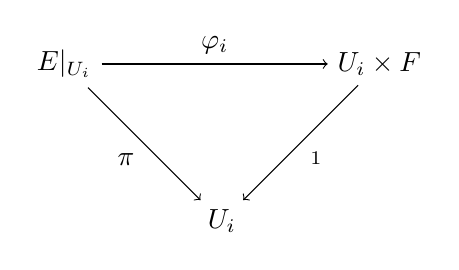
\begin{tikzpicture}
                \node (E) at (-2, 0) {$E|_{U_i}$};
                \node (UF) at (2, 0) {$U_i\times F$};
                \node (U) at (0, -2) {$U_i$};
                \draw[->] (E) -- node[above]{$\varphi_i$} (UF);
                \draw[->] (E) -- node[below left]{$\pi$} (U);
                \draw[->] (UF) -- node[below right]{$\pr_1$} (U);
            \end{tikzpicture}
        \end{gather*}
        It should be noted that the existence of such a cover is not a trivial matter. The general definition becomes quite involved when allowing for arbitrary smooth 2-spaces $B$. For convenience it will always be assumed that $B$ is an ordinary smooth space regarded as a 2-space with only trivial morphisms.

        As was the case in Definition \ref{bundle:fibre_bundle}, one can also characterize locally trivial 2-bundles by their transition data. Since the trivilizations $\varphi_i$ are equivalences, they admit an inverse (up to an invertible 2-map) and one can thus construct transition maps $\varphi_i\varphi_j^{-1}=U_{ij}\times F\cong U_{ij}\times F$ as usual. By the commutative diagram above, these transition maps only act on the fibre $F$. Because $\varphi_i\varphi_j^{-1}$ is itself an (auto)equivalence, the action on $F$ is given by a functor $g_{ij}:U_{ij}\rightarrow\mathrm{AUT}(F)$, where the 2-space $\mathrm{AUT}(F)$ is the \textit{coherent} 2-\textit{group}\footnote{Instead of the strict invertibility of maps in the definition of 2-groups above, one should allow for invertibility up to 2-isomorphisms that themselves satisfy certain coherence conditions.} of autoequivalences of $F$ together with invertible 2-maps between them.

        The interesting (and important) part is how the cocycle conditions \eqref{bundle:G_cocycle_condition} and \ref{bundle:G_cocycle_conditions} for the maps $g_{ij}$ are modified. Since the equivalences $g_{ij}$ are only invertible up to 2-maps, one cannot expect these conditions to hold as equations. Instead, two higher transition maps (i.e.~natural isomoprhisms) $h_{ijk}:g_{ij}\circ g_{jk}\Rightarrow g_{ik}$ and $k_i:g_{ii}\Rightarrow\text{id}_F$ are obtained. These higher data should in turn satisfy the necessary conditions coming from associativity and unitality constraints (similar to the coherence conditions from Section \ref{section:hda_group_cohomology}).
    }
    \newdef{$\mathcal{G}$-bundle}{\index{principal!bundle}
        A locally trivial 2-bundle with typical fibre $F$ is said to have the 2-group $\mathcal{G}$ as its structure (2-)group if the transition data factor through an action $\mathcal{G}\rightarrow\mathrm{AUT}(F)$. If $F=\mathcal{G}$, the 2-bundle is called a \textbf{principal $\mathcal{G}$-2-bundle}.
    }
    \begin{remark}[Gerbes]\index{gerbe}
        If the transition maps $k_i$ are chosen to be trivial and $\mathcal{G}$ is chosen to be respectively the trivial Lie 2-group associated to an Abelian Lie group $G$ or the automorphism 2-group of a Lie group $H$, one obtains Abelian and non-Abelian \textit{gerbes}. In fact, it can be shown that the 2-category of principal $2$-bundles is equivalent to the 2-category of gerbes for every Lie 2-group of the aforementioned type.
    \end{remark}

    By categorifying Definition \ref{bundle:holonomy_functor} of principal connections, one can define connections for principal $n$-bundles:
    \newdef{$n$-connection}{\index{connection!principal}
        Let $M$ be a smooth space and let $G$ be a Lie $n$-groupoid. Given a locally trivial principal $n$-bundle $P$ over $M$, an $n$-connection with $n$-holonomy is defined by the following data:
        \begin{itemize}
            \item for every coordinate chart $U_i\subset M$ a local holonomy $n$-functor
            \begin{gather}
                \mathrm{hol}_i:\mathcal{P}_n(U_i)\rightarrow G;
            \end{gather}
            \item for every double intersection $U_{ij}$ a 1-transfor (i.e.~an $n$-natural transformation)
            \begin{gather}
                g_{ij}:\mathrm{hol}_i\Rightarrow\mathrm{hol}_j;
            \end{gather}
            \item for every triple intersection $U_{ijk}$ a 2-transfor
            \begin{gather}
                f_{ijk}:g_{ij}\circ g_{jk}\Rrightarrow g_{ik};
            \end{gather}
            \item and so on...
        \end{itemize}
        This is equivalently given by a global $n$-functor
        \begin{gather}
            \mathrm{hol}:\mathcal{P}_n(M)\rightarrow\mathbf{Trans}_n(P).
        \end{gather}
    }

    ?? ADD GERBES (e.g.~BRYLINSKI) ??

\section{Space and quantity}

    In this section the general notions of spaces and observables are again considered. From the start everyhting will be formulated in an enriched setting where $\mathcal{V}$ is a cosmos \ref{cat:cosmos}. The categories $\mathbf{C}$ of interest will be assumed to be small.

    In the previous sections spaces modelled on a base space $X$, or more generally, on a category of spaces $\mathbf{S}$ were modelled as (concrete) sheaves on a suitable site. Here this notion is relaxed as much as possible:
    \newdef{Space}{\index{space}
        A (generalized) space modelled on a category $\mathbf{C}$ is a presheaf on $\mathbf{C}$.

        As before, the object $X(C)$ can be interpreted as the collection of ``probes'' from $C$ to $X$. The Yoneda lemma assures that ordinary test spaces in $\mathbf{C}$ can be viewed as spaces modelled on $\mathbf{C}$ and that their probes are indeed the ordinary maps in $\mathbf{C}$.
    }
    In a similar vein one can define observables as maps out of a space:
    \newdef{Quantity}{\index{quantity}
        A (generalized\footnote{It is generalized because it is ``measures'' a category instead of a single object.}) quantity on a category $\mathbf{C}$ is a copresheaf on $\mathbf{C}$.
    }

    \begin{property}[Isbell duality]\index{Isbell duality}
        Given a space $X$ one can look at the quantities that live on it (in ordinary geometry this would have been its algebra of functions). This defines a functor:
        \begin{gather}
            \mathcal{O}:\mathbf{Psh(C)}\rightarrow\mathbf{coPsh}^{op}(\mathbf{C}):X\mapsto\hom_\mathbf{Psh(C)}(X,\mathcal{Y}-).
        \end{gather}
        Similarly, given a quantity $Q$ one can ask on which space it behaves as the algebra of functions. This also defines as functor:
        \begin{gather}
            \mathrm{Spec}:\mathbf{coPsh}^{op}(\mathbf{C})\rightarrow\mathbf{Psh(C)}:Q\mapsto\hom_\mathbf{coPsh(C)}(\mathcal{Y}^{op}-,Q),
        \end{gather}
        where $\mathcal{Y}^{op}$ denotes the co-Yoneda embedding $\mathbf{C}\rightarrow\funccat{C}{\mathcal{V}}^{op}:c\mapsto\mathbf{C}(c,-)$.

        The incredible result is now that $(\mathcal{O}\dashv\text{Spec})$ is an adjunction, called the \textbf{Isbell adjunction}. Objects that are preserved (up to isomorphism) under the associated (co)monad are said to be \textbf{Isbell self-dual}.
    \end{property}
    \begin{example}[Cartesian spaces]
        When working over the site $\mathbf{CartSp}$ (with its usual topology) and restricting to coherent sheaves and product-preserving presheaves, the Isbell adjunction maps spaces to smooth algebras.
    \end{example}